\usepackage{fancyhdr}
\usepackage{amsmath,amsfonts,amsthm,amssymb,mathtools}
\usepackage{geometry}
\usepackage{etoolbox}
\usepackage{xifthen}
\usepackage{mathrsfs, graphics}
\usepackage{tikz}
\usepackage{tikzsymbols}
\usepackage{marginnote, xcolor}
\usepackage{graphicx}
\usepackage{footnote}
% \usepackage{fourier-orns}
% \usepackage{fontawesome5}
\usepackage{tcolorbox}
\tcbuselibrary{skins}

% Geometry

\geometry{a4paper, left=2cm, right=4cm}
\linespread{1.5}

% colors 

% \definecolor{denisBicep}{RGB}{216, 168, 146} 
% \definecolor{larratBicep}{RGB}{208, 153, 117} 
% \definecolor{graylol}{RGB}{144, 132, 124} 


\definecolor{denisBicep}{RGB}{26, 48, 146} 
\definecolor{larratBicep}{RGB}{78, 23, 97} 
\definecolor{graylol}{RGB}{44, 2, 14} 

% \definecolor{denisBicep}{RGB}{60, 48, 160} 
% \definecolor{larratBicep}{RGB}{0, 03, 70} 
% \definecolor{graylol}{RGB}{40, 200, 4} 

% fancy hdr

\pagestyle{fancy}                             

\newcommand{\lecture}[3]
{      
  
  \ifthenelse{\isempty{#3}}{
    \def\@lecture{Lecture #1\hfill#2}
    \def\ps{Lecture #1}
  }{
    \def\@lecture{Lecture #1: #3\tt\hfill#2}
    \def\ps{Lecture #1: #3}
  } 
  \subsection*{\@lecture}
}

\fancyhead[R]{\ps}
\fancyfoot[L]{\leftmark}
\fancyfoot[C]{}
\fancyfoot[R]{\thepage}

% general background

\newcommand{\divider}
{
	\begin{center}
	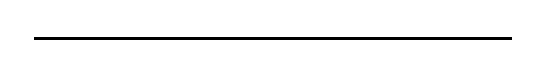
\begin{tikzpicture}
		\draw[thick, black] (0.25*\textwidth, 0) -- (0.75*\textwidth, 0);
		\node[rotate = 360 - 90, xshift = -0.6pt, yshift = 1pt] at (0.25*\textwidth,0){};
		\node[rotate = 90, xshift = -0.6pt, yshift = 1pt] at (0.75*\textwidth,0){};
	\end{tikzpicture}
	\end{center}
}

% new if definitions for chapter :c

\newif\ifchapterpage
\chapterpagefalse

% hook \chapter and then we set the flag :>

\let\oldchapter\chapter
\renewcommand{\chapter}{%
  \global\chapterpagetrue
  \oldchapter
}

\AddToHook{shipout/background}{
  \begin{tikzpicture}[remember picture, overlay]

    \ifchapterpage
    \draw[draw=black,fill=larratBicep!35, opacity=0.4] ([yshift = -(\paperheight - \textheight)/2 + 1.5cm, 
                                         xshift = (\paperwidth - \textwidth)/2 - 1.5cm]current page.north west) rectangle
                                          ([yshift = (\paperheight - \textheight)/2 + 0.5cm ,
                                          xshift = -(\paperwidth - \textwidth)/2 - 0.5cm]current page.south east);
    \draw[draw=larratBicep!50, step=5mm, opacity=0.4] ([yshift = -(\paperheight - \textheight)/2 + 1.5cm, 
                                          xshift = (\paperwidth - \textwidth)/2 - 1.5cm]current page.north west) grid
                                          ([yshift = (\paperheight - \textheight)/2 + 0.5cm ,
                                          xshift = -(\paperwidth - \textwidth)/2 - 0.5cm]current page.south east);
    \draw[draw=black] ([yshift = -(\paperheight - \textheight)/2 + 1.5cm, 
                                         xshift = (\paperwidth - \textwidth)/2 - 1.5cm]current page.north west) rectangle
                                         ([yshift = (\paperheight - \textheight)/2 + 0.5cm ,
                                         xshift = -(\paperwidth - \textwidth)/2 - 0.5cm]current page.south east);
      \global\chapterpagefalse

    \else         

    \draw[draw=black,fill=larratBicep!35, opacity=0.4] ([yshift = -(\paperheight - \textheight)/2 + 1.5cm, 
                                         xshift = (\paperwidth - \textwidth)/2 - 1.5cm]current page.north west) rectangle
                                          ([yshift = (\paperheight - \textheight)/2 + 0.5cm ,
                                          xshift = -(\paperwidth - \textwidth)/2 - 0.5cm]current page.south east);
    \draw[draw=larratBicep!50, step=5mm, opacity=0.4] ([yshift = -(\paperheight - \textheight)/2 + 1.5cm, 
                                          xshift = (\paperwidth - \textwidth)/2 - 1.5cm]current page.north west) grid
                                          ([yshift = (\paperheight - \textheight)/2 + 0.5cm ,
                                          xshift = -(\paperwidth - \textwidth)/2 - 0.5cm]current page.south east);
    \draw[draw=black] ([yshift = -(\paperheight - \textheight)/2 + 1.5cm, 
                                         xshift = (\paperwidth - \textwidth)/2 - 1.5cm]current page.north west) rectangle
                                         ([yshift = (\paperheight - \textheight)/2 + 0.5cm ,
                                         xshift = -(\paperwidth - \textwidth)/2 - 0.5cm]current page.south east);
    \fi

  \end{tikzpicture}
}

% parenthesis check

\newcommand{\maybep}[1]{ 
  \if\relax\detokenize{#1}\relax
  \else
    \ (#1)
  \fi
}

% tcolorbox environments

\usetikzlibrary{patterns}

\newtcolorbox[auto counter, number within=section]{theorem}[1][]           
{title=Theorem \thetcbcounter\maybep{#1}: ,drop lifted shadow=black,enhanced,colframe=blue!50!black,colback=blue!25!denisBicep!50,attach title to upper = {\ },
coltitle=blue!50!black,fonttitle=\upshape\bfseries,fontupper=\itshape,
sharp corners = all,boxrule = 0pt,
underlay = {\draw[step=5mm,
  draw = blue!25!denisBicep!60] (interior.north east)
grid (interior.south west);
\draw[blue!25!denisBicep!60] ([xshift = 0.45cm]interior.north west) -- ([yshift = -0.28cm, xshift = 0.48cm]interior.north west); %  -----
\draw[blue!25!denisBicep!60] ([yshift = -0.35cm]interior.north west) -- ([yshift = -0.28cm, xshift = 0.48cm]interior.north west); % -
\path[fill = blue!40!denisBicep!40,drop shadow={opacity = 0.55, shadow xshift = .0ex, shadow yshift = -.4ex, shadow scale = 1, 
 }]
([xshift = 0.45cm]interior.north west) -- ([yshift = -0.28cm, xshift = 0.48cm]interior.north west) -- 
   ([yshift = -0.35cm]interior.north west) -- ([xshift = 0.45cm]interior.north west) ;
                                                                                                                              % -  x
\fill[fill=larratBicep!35] ([yshift = -0.35cm]interior.north west) -- ([xshift = 0.45cm]interior.north west) -- (interior.north west);

\draw[larratBicep!50] ([yshift = -0.35cm]interior.north west) -- (interior.north west);
\draw[larratBicep!35] ([yshift = -0.35cm]interior.north west) -- ([xshift = 0.45cm]interior.north west);
\draw[larratBicep!35] ([xshift = 0.45cm]interior.north west) -- (interior.north west);
}
}

\newtcolorbox[use counter from=theorem]{proposition}[1][]           
{title=Proposition \thetcbcounter\maybep{#1}: ,drop lifted shadow=black,enhanced,colframe=denisBicep!35,colback=denisBicep!35,attach title to upper = {\ },
underlay = { 
  \draw[larratBicep!60] ([xshift = 0.45cm]interior.north west) -- ([yshift = -0.28cm, xshift = 0.48cm]interior.north west); %  -----
  \draw[larratBicep!60] ([yshift = -0.35cm]interior.north west) -- ([yshift = -0.28cm, xshift = 0.48cm]interior.north west); % -
  \path[fill = larratBicep!45,drop shadow={opacity = 0.55, shadow xshift = .0ex, shadow yshift = -.4ex, shadow scale = 1, 
   }]
  ([xshift = 0.45cm]interior.north west) -- ([yshift = -0.28cm, xshift = 0.48cm]interior.north west) -- 
     ([yshift = -0.35cm]interior.north west) -- ([xshift = 0.45cm]interior.north west) ;
                                                                                                                                % -  x
  \fill[fill=larratBicep!35] ([yshift = -0.35cm]interior.north west) -- ([xshift = 0.45cm]interior.north west) -- (interior.north west);

  \draw[larratBicep!50] ([yshift = -0.35cm]interior.north west) -- (interior.north west);
  \draw[larratBicep!35] ([yshift = -0.35cm]interior.north west) -- ([xshift = 0.45cm]interior.north west);
  \draw[larratBicep!35] ([xshift = 0.45cm]interior.north west) -- (interior.north west);
},
coltitle=red!50!black,fonttitle=\upshape\bfseries,fontupper=\itshape,
sharp corners = all,boxrule = 0pt,
underlay = {\draw[step=5mm,
  draw = larratBicep!45] (interior.north east)
grid (interior.south west);}
}

\newtcolorbox[auto counter, number within=section]{definition}[1][]           
{title=Definition \thetcbcounter\maybep{#1}: ,drop lifted shadow=black,enhanced,colframe=red!25,colback=red!25!larratBicep!50,attach title to upper = {\ },
coltitle=red!50!black,fonttitle=\upshape\bfseries,fontupper=\itshape,
sharp corners = all,boxrule = 0pt,
underlay = {\draw[step=5mm,
  draw = red!25!larratBicep!60] (interior.north east)
grid (interior.south west);
  \draw[red!35] ([xshift = 0.45cm]interior.north west) -- ([yshift = -0.28cm, xshift = 0.48cm]interior.north west); %  -----
  \draw[red!35] ([yshift = -0.35cm]interior.north west) -- ([yshift = -0.28cm, xshift = 0.48cm]interior.north west); % -
  \path[fill = red!35,drop shadow={opacity = 0.55, shadow xshift = .0ex, shadow yshift = -.4ex, shadow scale = 1, 
   }]
  ([xshift = 0.45cm]interior.north west) -- ([yshift = -0.28cm, xshift = 0.48cm]interior.north west) -- 
     ([yshift = -0.35cm]interior.north west) -- ([xshift = 0.45cm]interior.north west) ;
                                                                                                                                % -  x
  \fill[fill=larratBicep!35] ([yshift = -0.35cm]interior.north west) -- ([xshift = 0.45cm]interior.north west) -- (interior.north west);

  \draw[larratBicep!50] ([yshift = -0.35cm]interior.north west) -- (interior.north west);
  \draw[larratBicep!35] ([yshift = -0.35cm]interior.north west) -- ([xshift = 0.45cm]interior.north west);
  \draw[larratBicep!35] ([xshift = 0.45cm]interior.north west) -- (interior.north west);
}
}

\usetikzlibrary{shadows}
\newtcolorbox[use counter from=theorem]{corollary}[1][]           
{title=Corollary \thetcbcounter\maybep{#1}: ,drop lifted shadow=black,enhanced,colframe=green!35!black!15,colback=green!35!black!15!denisBicep!45,attach title to upper = {\ },
coltitle=green!25!black,fonttitle=\upshape\bfseries,fontupper=\itshape,
sharp corners = all,boxrule = 0pt,
underlay = {\draw[step=5mm,
  draw = green!40!black!30!denisBicep!50] (interior.north east)
grid (interior.south west);

  \draw[green!40!black!35] ([xshift = 0.45cm]interior.north west) -- ([yshift = -0.28cm, xshift = 0.48cm]interior.north west); %  -----
  \draw[green!40!black!35] ([yshift = -0.35cm]interior.north west) -- ([yshift = -0.28cm, xshift = 0.48cm]interior.north west); % -
  \path[fill = green!35!black!20,drop shadow={opacity = 0.55, shadow xshift = .0ex, shadow yshift = -.4ex, shadow scale = 1, 
   }]
  ([xshift = 0.45cm]interior.north west) -- ([yshift = -0.28cm, xshift = 0.48cm]interior.north west) -- 
     ([yshift = -0.35cm]interior.north west) -- ([xshift = 0.45cm]interior.north west) ;
                                                                                                                                % -  x
  \fill[fill=larratBicep!35] ([yshift = -0.35cm]interior.north west) -- ([xshift = 0.45cm]interior.north west) -- (interior.north west);

  \draw[larratBicep!50] ([yshift = -0.35cm]interior.north west) -- (interior.north west);
  \draw[larratBicep!35] ([yshift = -0.35cm]interior.north west) -- ([xshift = 0.45cm]interior.north west);
  \draw[larratBicep!35] ([xshift = 0.45cm]interior.north west) -- (interior.north west);
}
}

\newtcolorbox[auto counter]{example}
{title=Example: ,drop fuzzy shadow=black,enhanced,colframe=gray!50!black,colback=gray!35,attach title to upper = {\ },
coltitle=gray!50!black,fonttitle=\upshape\bfseries,fontupper=\itshape,
sharp corners = all,boxrule = 0pt,
underlay = {\draw[step=5mm,
  draw = gray!40!black!30] (interior.north east)
grid (interior.south west);}
}

% margi note configuration

\makeatletter

\setlength{\marginparsep}{18pt}
\renewcommand*{\marginfont}{\color{blue}}
\makeatother

% other (exercise enviroment)

\newcommand{\exercise}[1][]{
    \def\@exercise{#1}
    \subsection*{Exercise #1}
}

\newcommand{\subexercise}[1][]{
    \subsubsection*{Exercise \@exercise.#1}
}

% macros

\newcommand{\integral}[4]{\int\limits_{#1}^{#2} #4 d#3}
\newcommand{\limit}[3]{\lim\limits_{#1 \rightarrow #2} #3}
\newcommand{\strone}[2]{\left[ \begin{gathered}#1\\ #2\end{gathered} \right] }
\newcommand{\strtwo}[2]{\left\{ \begin{gathered}#1\\ #2\end{gathered} \right\} }
\newcommand{\strthree}[2]{\left\lfloor \begin{gathered}#1\\ #2\end{gathered} \right\rfloor }

\newcommand{\startbf}[1]{\text{\bfseries{#1}}}
\newcommand{\sett}[1]{\left\{ #1 \right\}}
\newcommand{\thesis}[1]{\left( #1 \right)}
\newcommand{\brkt}[1]{\left[ #1 \right]}
\newcommand{\floor}[1]{\left\lfloor #1 \right\rfloor}

\DeclareMathOperator{\img}{im} 
\DeclareMathOperator{\Img}{Im} 
\DeclareMathOperator{\coker}{coker} 
\DeclareMathOperator{\Coker}{Coker} 
\DeclareMathOperator{\Ker}{Ker} 
\DeclareMathOperator{\rank}{rank}
\DeclareMathOperator{\Spec}{Spec} 
\DeclareMathOperator{\Tr}{Tr} 
\DeclareMathOperator{\pr}{pr} 
\DeclareMathOperator{\ext}{ext} 
\DeclareMathOperator{\pred}{pred} 
\DeclareMathOperator{\dom}{dom} 
\DeclareMathOperator{\ran}{ran} 
\DeclareMathOperator{\Hom}{Hom} 
\DeclareMathOperator{\Mor}{Mor} 
\DeclareMathOperator{\End}{End} 

\newcommand{\lm}{\ensuremath{\lambda}}
\newcommand{\eps}{\ensuremath{\epsilon}}
\newcommand{\veps}{\ensuremath{\varepsilon}}
\newcommand{\al}{\ensuremath{\alpha}}
\newcommand{\bb}{\ensuremath{\beta}}
\newcommand{\cc}{\ensuremath{\gamma}}
\newcommand{\dd}{\ensuremath{\delta}}
\newcommand{\DD}{\ensuremath{\Delta}}
\newcommand{\ff}{\ensuremath{\phi}}
\newcommand{\FF}{\ensuremath{\varphi}}

\newcommand{\RR}{\mathbb{R}}
\newcommand{\RO}{\mathcal{R}}
\newcommand{\EE}{\mathbb{E}}
\newcommand{\CC}{\mathbb{C}}
\newcommand{\RW}{\mathbb{R}^2}
\newcommand{\RT}{\mathbb{R}^3}
\newcommand{\RN}{\mathbb{R}^n}
\newcommand{\DS}{\mathcal{D}}

\newcommand{\KK}{\mathbb{K}}
\newcommand{\KW}{\mathbb{K}^2}
\newcommand{\KT}{\mathbb{K}^3}
\newcommand{\KN}{\mathbb{K}^n}

\newcommand{\NN}{\mathbb{N}}

\newcommand{\PS}{\mathcal{P}}
\newcommand{\AS}{\mathcal{E}}
\newcommand{\FS}{\mathcal{F}}
\newcommand{\LS}{\mathcal{L}}
\newcommand{\MS}{\mathcal{M}}
